% For MISTA 2015, use the default option that has been supplied
\documentclass{svjour3}                     % onecolumn (standard format)
%\documentclass[smallextended]{svjour3}     % onecolumn (second format)
%\documentclass[twocolumn]{svjour3}         % twocolumn
%
\smartqed  % flush right qed marks, e.g. at end of proof
%
\usepackage{graphicx}
\usepackage{amsmath,amssymb}
\usepackage{listings}
\usepackage{colortbl}

\lstset{frame=tb,
  language=Java,
  aboveskip=3mm,
  belowskip=3mm,
  showstringspaces=false,
  columns=flexible,
  basicstyle={\small\ttfamily},
  numbers=none,
  breaklines=true,
  breakatwhitespace=true,
  tabsize=3
}


%
% \usepackage{mathptmx}      % use Times fonts if available on your TeX system
%
% insert here the call for the packages your document requires
%\usepackage{latexsym}
% etc.
%
% please place your own definitions here and don't use \def but
% \newcommand{}{}
%
% Insert the name of "your journal" with
% This is preset for MISTA 2015: Do not change
\journalname{MISTA 2015}
%


\begin{document}

\title{Model for planning of distributed data production}

\author{Dzmitry Makatun         \and
		J\'er\^ome~Lauret		\and
		Hana~Rudov\'a			\and
		Michal~\v{S}umbera	
}

\institute{Dzmitry Makatun \at
              Faculty of Nuclear Physics and Physical Engineering, Czech Technical University in Prague \\
              \email{makatun@rcf.rhic.bnl.gov}           %  \\
           \and
           J\'er\^ome~Lauret \at
              STAR, Brookhaven National Laboratory (BNL), USA \\
              \email{jlauret@bnl.gov}          %  \\              
           \and
           Hana~Rudov\'a \at
              Faculty of Informatics, Masaryk University, Brno, Czech Republic \\
              \email{hanka@fi.muni.cz}           %  \\              
           \and
           Michal~\v{S}umbera \at
              Nuclear Physics Institute (NPI), Academy of Sciences (ASCR),
 Czech Republic \\
              \email{sumbera@ujf.cas.cz}           %  \\
}

\maketitle
\section{Introduction}
\label{intro}
The STAR experiment at the Relativistic Heavy Ion Collider (RHIC) studies a
primordial form of matter that existed in the universe shortly after the Big
Bang. Collisions of heavy ions occur millions of times per second inside the
detector, producing tens of petabytes of raw data each year. All the raw data
has to be processed in order to reconstruct physical events which are
further analyzed by scientists. This process is called data production.  Like
any other modern experiment in High Energy and Nuclear Physics (HENP), STAR intends to rely on
distributed data processing, making use of several remote computational sites
(for some experiments this number can scale up to several hundreds).

When running data intensive applications on distributed computational
resources long I/O overheads may be observed as access to remotely stored data
is performed. Latency and bandwidth can become the major limiting factors for
the overall computation performance and can reduce the CPU time\,/\,wall time 
ratio due to excessive I/O wait. 
Widely used data management systems in the HENP community
(Xrootd, DPM) are focused on providing heterogeneous access to distributed
storage and do not consider data pre-placement with respect to available CPUs,
job duration or network performance. At the same time job scheduling systems
(PBS, Condor) do not reason about transfer overheads when accessing data at
distributed storage. For this reason, an optimization of data transferring and
distribution across multiple sites is often done manually, using a custom
setup for each particular infrastructure \cite{Balewski}. 

In previous collaboration between BNL and NPI/ASCR, the problem of
efficient data transferring in a Grid environment was addressed \cite{Zerola}.
% and cache management \cite{Makatun_cache}. 
Data transfers between $n$~computational sites and $m$~data locations were
considered but job scheduling was not covered
by that work. In \cite{ACAT_cp} we
proposed a constraint programming planner that schedules computational jobs
and data transfers in a distributed environment in order to optimize resource
utilization and reduce the overall completion time. Since such global
scheduling is computationally demanding it should be divided into several
stages in order to improve scheduler performance and scalability. A planning of
resource load can be completed in the first stage before scheduling file
transfers and jobs. In this work we address the problem of data production
planning, answering the question how the data should be transferred given the
network structure, bandwidth, storage and CPU slots available. This will allow
local schedulers to process jobs and have CPUs busy all the time while not
exceeding disk and network capacities.

Optimization of data intensive applications in Grid was studied
in~\cite{Globus_scheduler}. In this work an optimization was achieved by
replication of highly used files to more sites while the jobs were executed
where their input data is located. However, this is not the case for data
production, when each file has to be processed once. 
%
Explicit model distributing jobs over a Grid with respect to the network
bandwidth was proposed in~\cite{Trees}. The network structure of the Grid was
modeled as a tree and all the files were assumed to be of the same size and
processing time. In our study we do not limit the network topology to trees,
and assume fluctuations of job parameters. 

\section{Modeling}
\label{modeling}
Due to a data level of parallelism a typical workflow of HENP computation
consists of independent jobs using one CPU, one input and one output file. We
assume there is a local scheduler running at each site, which picks a new
input file to process from the local storage of that site each time when a CPU becomes
free. Input data must be transferred from the central storage
to each site in such a manner that at the every moment of time there is enough
input files at each site to keep all the available CPUs busy while not
exceeding the local storage and network throughput. Another task
is to transfer the output files back to central storage, cleaning each local
storage for the new input.

Let us consider a scheduling time interval $\Delta T$. We assume that at the
starting moment all the CPUs in the Grid are busy, and there is some amount of
input data already placed at each site. We need to transfer the next portion
of data to each site during time interval $\Delta T$ in order to avoid
draining of the local queue by the end of this interval. 

The computational Grid is represented by a directed weighted graph where
vertexes $c_{i} \in C$ are computational nodes and edges $l_{j} \in L$ are
network links. The weight of each link $b_{j}$ is the amount of data that can be
transferred over the link per unit of time (i.e. bandwidth). One of the nodes
$c_{0}$ is the central storage where all the input files for the further
processing are initially placed. All the output files has to be transferred
back to $c_{0}$ from the computational nodes. We will give two separate
problem formulations: for an input and output transfer planning. 

In order to formulate a network flow maximization problem \cite{Network_flows}
for input/output file transferring we have to define a capacitated $\{s,t\}$
network, which is a set of vertexes $V$ including a source $s$ and a sink $t$;
and a set of edges $e\in E$ with their capacities $cap(e)$. A solution that
assigns a non-negative integer number $f(e)$ to each edge $e \in E$ can be
found in polynomial time with known algorithms.

\subsection{Input flow planning}
\begin{figure}[h]
	\begin{center}
		\includegraphics [trim= 30mm 20mm 30mm 30mm , clip, angle =-90, width=0.7\textwidth]{pic/network_general.pdf}
	\end{center}
	\caption{Data production Grid represented as an capacitated $\{s,t\}$ network for input transfer planning (general case). $c_{0}$ is a central NFS storage (Tier-0), $c_{i}$ are computational nodes (where $i>0$), $l_{j}$ are network links, $d_{i}$ are dummy edges from computational nodes to the sink $t$, $q_{0}$ is a dummy edge leading from the source $s$ to the $c_{0}$. }
	\label{network_general}
\end{figure}  
In order to transform a given graph of a Grid into a capacitated $\{s,t\}$
network for an input transfer problem (see Figure \ref{network_general})we add two dummy vertexes: a source $s$
and a sink $t$. Next we add  dummy edges $d_{i} \in D$ from each computational
node $i$ to the sink, and a dummy edge $q_{0}$ from the source $s$ to the
central storage $c_{0}$. These dummy edges allow us to introduce constraints
on the storage capacity of the nodes. The set of vertexes $V$ consists of
computational nodes $C$ and dummy vertexes: $V= C \cup \{s,t\}$. The final set
of edges consists of real network links $L$, dummy edges $D$ from
computational nodes to the sink and from the source to the central storage
$q_{0}$: $E= L \cup D \cup \{q_{0}\}$. Capacity of each edge defines the
maximal amount of data that can be transferred over an edge within time
interval $\Delta T$: 
%
\begin{equation} 
\label{edge_cap} 
cap(e) = \left\{
\begin{array}{l l} 
b_{j} \cdot \Delta T & \text{if }e = l_{j} \in L \\ w_{i} &
\text{if } e = d_{i} \in D\\ k_{0} & \text{if } e = q_{0} 
\end{array} \right.
\end{equation} 
%
where $w_{i}$ is the maximal amount of data that can be
transferred to the node $i$ without exceeding its storage capacity $Disk_{i}$
and $k_{0}$ is the total size of available input files at $c_{0}$. We denote
the solution for the input transfer problem as $f^{in}(e)$.

\subsection{Output flow planning}

\label{outproblem}
\begin{figure}[h]
	\begin{center}
		\includegraphics [trim= 30mm 20mm 30mm 30mm , clip, angle =-90, width=0.7\textwidth]{pic/network_general_out.pdf}
	\end{center}
	\caption{Data production Grid represented as an capacitated $\{t,s\}$ network for output transfer planning (general case). $c_{0}$ is a central NFS storage (Tier-0), $c_{i}$ are computational nodes (where $i>0$), $l_{j}$ are network links, $\overline{d}_{i}$ are dummy edges from the source $t$ to computational nodes, $\overline{q}_{0}$ is a dummy edge leading from $c_{0}$ to the sink $s$. }
	\label{general_out}	
\end{figure}

For transfer of output files we use a similar transformation, but swap the
source $s$ and the sink $t$, change the direction of dummy edges and redefine
capacities of dummy edges (see Figure \ref{general_out}). In this case the capacity $\overline{k}_{0}$ of the
dummy edge $\overline{q}_{0}$ leading from the central storage $c_0$ to the
sink $s$ is equal to the amount of data which can be transferred to $c_0$
within time interval $\Delta T$ (it is limited by the available space at the
central storage). The capacity $\overline{w}_{i}$ of dummy edges
$\overline{d}_{i}$ leading from the source $t$ to computational nodes $c_{i}$
is equal to the maximum amount of output data which can be transferred from
the node $c_{i}$.
%
\begin{equation}
\label{edge_cap_out}
cap(e) = \left\{ 
  \begin{array}{l l}
    b_{j} \cdot \Delta T & \text{if }e = l_{j} \in L \\
    \overline{w}_{i} & \text{if } e = \overline{d}_{i} \in \overline{D}\\
    \overline{k}_{0} & \text{if } e = \overline{q}_{0}
  \end{array} \right.
\end{equation}
%
We denote the solution for the output transfer problem as $f^{out}(e)$.

\subsection{Capacities of dummy edges}
Let us consider data production jobs which perform the same type of processing
on the same type of files. Duration $p_{j}$ of a job $j$  processing an input
file of size $InSize_{j}$ at a node $i$ is $p_{j} = \alpha_{i} \cdot
InSize_{j}$ where $\alpha_{i}$ is constant for each node $i$.  The ratio of
size of input $InSize_{j}$ and output $OutSize_{j}$ files of each job $j$ is
considered to be constant for the same type of data processing, i.e.,
$OutSize_{j} = \beta \cdot InSize_{j}$.  During the time interval $\Delta T$ a
node $i$ with $NCPU_{i}$  of CPUs  will process $\frac{1}{\alpha_{i}} \cdot
NCPU_{i} \cdot \Delta T$ of input data and will produce
$\frac{\beta}{\alpha_{i}} \cdot NCPU_{i} \cdot \Delta T$ of output data.
Using constraints on storage space, we can define the maximal amount of input
$w_{i}$ and output $\overline{w}_{i}$ data which can be transferred to/from a
node $i$:
%
\begin{eqnarray}
w_{i} &=&
Disk_{i} - I_{i}^{in} - I_{i}^{out} + \frac{1 - \beta}{\alpha_{i}} \cdot
NCPU_{i} \cdot \Delta T + Del_{i}^{out} \label{w}\\
\overline{w}_{i} &=& I_{i}^{out} + \frac{\beta}{\alpha_{i}} \cdot NCPU_{i} \cdot \Delta T - Min_{i}^{out} \label{sigma}
\end{eqnarray}  
%
where $Disk_{i}$ is available disk space at the node $i$, $I_{i}^{in}$ and
$I_{i}^{out}$ are the initial size of input and output data at a local storage
respectively, $Del_{i}^{out}$ is the amount of output data that will be
transferred out of the node and deleted from its storage during $\Delta T$;
$Min_{i}^{out}$ is the total size of output files which cannot be transferred
because the jobs which produce them are not finished (output files of running
jobs). 

In the Eqn.~\ref{w}, $Del_{i}^{out}$ is equal to the amount of data which will
be transferred from a node $c_{i}$, i.e., the solution to the output transfer
problem $f^{out}(\overline{d}_{i})$. In the Eqn.~\ref{sigma}, $\Delta T$ and
$Min_{i}^{out}$ are parameters of the scheduler. The other values used in
Eqns.~\ref{w}--\ref{sigma} can be obtained from monitoring data right before
each planning iteration.

\section{Solving Procedure}
\label{solve}

It can be proven that the maximum flow problems for input and output transfers
can be solved independently under assumptions: (a) all the real network links
in the considered Grid are full-duplex, i.e., a network throughput between two
nodes is the same in both directions (b) in a steady state the size of the
output transferred from each node is proportional to the size of the input
transferred to that node in each scheduling interval, i.e.,
$f^{out}(\overline{d}_{i})= \beta \cdot f^{in}(d_{i})$, where $\beta \leq 1$.

Since in real environment the assumption (b) will not strongly hold due to
resource performance fluctuations we propose the following approach to
solve the problem:
%
\begin{enumerate}
\item Calculate values for $\overline{w}_{i}$ using Eqn.~\ref{sigma}.
\item Solve the problem for output data flows to obtain $f^{out}(e)$.
\item Using Eqn.~\ref{w} and $Del_{i}^{out} = f^{out}(\overline{d}_{i})$ calculate $w_{i}$.
\item For real links $l \in L$ reduce the capacity by the amount which is used by output transfers: $cap(l_{j}) = b_{j} \cdot \Delta T - f^{out}(l_{j})$.
\item Solve the problem for input transfers with $w_{i}$ and $cap(l_{j})$ defined in previous steps. Find input data flows $f^{in}(e)$.
\end{enumerate}
%
To conclude, this procedure is expected to compute feasible data transfers 
such that CPUs in Grid are busy with computational jobs while not exceeding 
local disk capacities.

\subsection{Plan execution}
\label{plan-execution}
After the global plan was created it has to be executed by computational
nodes. For that we assume that there is a dedicated service running at each node
which is responsible for sending statistics to the global planing, receiving the plan and executing it. We call such a service a local \textbf{ handler}. 

The local handler keeps counters of how much data of each type remains to be send from this node to each  possible destination during the current plan iteration. This implies two counters (input and output) for each outgoing link. When the handler receives a new global plan it updates the counters to be equal to the flows of corresponding edges. If the handler has not managed to send/receive all the data according to the global plan within the time window, the system will automatically recover from such an error, since each planing iteration relay on the current state of the system, but not on previously issued plans.  

For the plan execution, each time when a new file arrives to the node, the handler decides either to keep the file for local processing or to forward it to another node. In order to make the decision the handler executes the first satisfied alternative from the following list:

\begin{enumerate}
\item If the received file is of input type and if there is a free CPU at the node $\Rightarrow$ submit the file for processing.
\item If there is a destination with a greater-than-zero counter for the corresponding file type $\Rightarrow$ transfer the file to that destination. Decrease the counter by the size of the file.
\item Keep the file at the local storage until it can be processed (when a CPU becomes free  or a new plan arrives).
\end{enumerate}
Such an order of alternatives ensures that the file will be processed as soon as it arrives to the node with a free CPU, and all the CPUs will be busy as long as there are unprocessed input files at the node. Since an input file will not be forwarded unless all the CPUs are busy, no excessive transfers will happen in the system.

Another important role of the handler is to check the consistency of each file upon receive and send the confirmation to the sender node. Only after the confirmation the file can be deleted from the sender node, otherwise data loss may emerge. 

When processing of an input file starts, the handler makes a reservation for the whole output file, and when it is finished - deletes the input file.
\section{Simulations}
\subsection{Simulation setup}
In our experiments the "Grid Simulation Toolkit For Resource Modelling And Application Scheduling For Parallel And Distributed Computing" (GridSim) \cite{GridSim} was used for realistic simulations of distributed data production. It is a discrete-event simulation toolkit which provides extensive models of computational clusters, job scheduling and execution, network, data transferring and etc. Additional functionality for global plan execution \ref{plan-execution}, statistics collection and a simple storage management was implemented on top of the GridSim package for our simulations.

Sending files over the network is an essential part of our simulations, while it is briefly described below, the detailed description can be found in \cite{GridSimNetwork}. When a simulated entity (i.e. computational node) executes a "transfer the file" command, the file is stored to the output queue and then it is processed by underlying network model. If there are several networks links connected to the entity, then each of them has its own queue. Two file transfer modes were used:
\begin{itemize}
\item \textbf{Sequential:} files are transferred one by one in the order as they appear in the queue, only one transfer at a time is performed. 
\item \textbf{Parallel:} all the files in queue are being transferred simultaneously, sharing the bandwidth.  In particular, newly started transfers delay those in progress.
\end{itemize}
An important consequence of the difference between the two modes appears when an entity sends a set of multiple files to the same destination simultaneously. In both modes the complete transfer time of a file set will be the same, but in the \textbf{sequential} transfer mode the files will arrive one by one and the first file will become available faster than in the \textbf{parallel} transfer mode, where the delay of the first file will depend on size of the set. A comparison study of parallel / sequential transfer modes in real network can be found in \cite{Zerola}, where the authors has shown that transferring files sequentially (but using multiple threads) can be advantageous for HENP computations compared to parallel transfer of multiple files. However, due to various aspects, the parallel transfer mode is a more common model for distributed data processing in HENP.

In order to test our planning model against other approaches, we have simulated distributed data production under the scheduling scenarios listed below. In all the scenarios, the input data is initially placed at the central storage and all the output data has to be transferred back to it, all the CPUs in the system are free at the initial moment of time.
\begin{itemize}
\label{scenarios}
\item \textbf{PLANER:}  This scenario uses the global planing described in our model. The \textit{sequential transfer network} mode is used as the preferable one. 
\item \textbf{PUSH\_par:} Whenever there is a free CPU in the Grid, the central storage sends next input file to the computational node with this free CPU. When a node receives an input file, it starts processing, and after it is finished it sends the output file back to the central storage. When the central storage receives an output file it is informed that a CPU became free at the sender node. In such a manner, the central storage keeps sending input files until all the data are processed. The shortest network path is used for file transfers. The \textit{parallel transfer network} mode is used here, which leads to uncoordinated concurrent access to remote files by simultaneous jobs. This scenario is the closest to the distributed data production setup in many HENP experiments, in particular, data production at KISTI for the STAR experiment \cite{KISTI-production}. 
\item \textbf{PUSH\_seq:} The job scheduling in performed exactly as in the previous scenario, but the \textit{sequential transfer network} mode is used. The main purpose of these simulations is to study the effects of sequential file transferring on the data production and, also, to estimate which part of the performance improvement in the PLANER scenario is achieved by the sequential transferring alone.
\item \textbf{no\_network:} Again, the job scheduling is the same as in two previous scenarios, but the network is not considered here. The production is performed as if all the CPUs are aggregated at the single site and can read/write the data directly from/to the storage with no latency. This scenario serves as a base case for comparison. It allows to estimate the limit for the processing makespan, and estimate the influence of the transfer latency. Obviously, none of the other scenarios can process the data faster than the one with no network delay.
\end{itemize}


The main metrics used for performance comparison is the makespan, which is calculated as time passed from the start of the first input file transfer from the central storage until the finish time of the last output file transfer to it. For comparison of two scheduling policies, a makespan improvement can be calculated as follows:


\begin{equation}
\label{makespanImprovement}
 makespan~improvement = \frac{makespan_{1} - makespan_{2}}{makespan_{1}} 
\end{equation}

\subsection{Using data from real data production systems}

A remote data production of the experiment STAR was ongoing at the computational facility of the Korea Institute of Science and Technology Information (KISTI)\cite{KISTI} for seven months in 2014. The log database of the data production framework contains information on job durations, sizes of input and output. Records of 60 000 computational jobs were taken from log an used as input for our simulations. The average parameters of the set of jobs are provided in Table \ref{tab:jobs}.

\begin{table}
\caption{Parameters of 60000 data production jobs recovered from log database of data production framework and used for simulations. The data production was setup at KISTI computing facility for the STAR experiment and continued for 7 months in 2014.}
\label{tab:jobs}
\begin{center}
\begin{tabular}{ l  c  r  r  r	|r }
\hline %\hline
% \br                   
  Parameter  & Units& Average & Min & Max & Total \\ \hline %\mr 
  Duration & hours & 46 & 12&64&314 (years) \\ 
  Input file size & MB & 4320& 895&4780&259 (TB) \\	
  Output file size & MB & 3022& 105&3614&181(TB) \\
  $\alpha$ & s/MB & 38& 9&105&- \\
  $\beta$ & - & 0.7& 0.02& 1.9&-\\	
  \hline %\hline
 % \br 
\end{tabular}
    \end{center}
\end{table}

In order to setup realistic parameters of simulated computational nodes, two sources were considered: the data production framework at KISTI \cite{KISTI-production}; and the online monitoring system of the ALICE experiment at CERN (MonAlisa) \cite{MonAlisa}. According to the second source, the number of CPUs available at remote nodes can vary from several units up to several thousands, while typical values for interconnecting network bandwidth are $\sim 50$ Mbps $- 2 $Gbps. More detailed setup description for each particular simulation is given in the following subsections. 

\subsection{Simulations with one remote node}
In the first set of simulations we aimed to reproduce the remote data production of the experiment STAR at KISTI computing facility. The environment consisted of a single remote computational node connected to the central storage. While the in real setup the number of CPUs at the remote site was 1000 CPUs and the network bandwidth was $\sim1$ Gbps \cite{KISTI-production}, we did simulations with a wide scope of these parameters in order to study their influence on the computational efficiency. By simulations with a single remote node, we would like to address the following questions: is the proposed model able to provide efficient data pre-staging at the remote node? How does the required bandwidth depends on the number of CPUs at the remote site? How many CPUs at the remote site can be exploited efficiently, given the network bandwidth?

%---------------Bandwidth-------------------------
\begin{figure}[h]
\centering
\begin{minipage}{.7\textwidth}
\centering
    \includegraphics[trim =00mm 00mm 00mm 00mm ,clip, width=1\textwidth]{pic/1node_relative_makespan.pdf}

    \caption{Dependence of makespan on network bandwidth for one remote node with 1000 CPUs}
    \label{1node_relative_makespan}
\end{minipage}\hspace{1pc}%
\begin{minipage}{.7\textwidth}
\centering
    \includegraphics[trim =00mm 00mm 00mm 00mm ,clip, width=1\textwidth]{pic/1node_makespan_improvement.pdf}
    \caption{Makespan improvement of proposed model compared to PUSH\_par and PUSH\_seq}
    \label{1node_makespan_improvement}
\end{minipage} 
\end{figure}


The Figures \ref{1node_relative_makespan} and \ref{1node_makespan_improvement} present results of simulations where the number of CPUs at the remote site was 1000, the size of its storage was 12 TB and the network bandwidth was changing from 50 Mbps to 2 Gbps in different simulation runs. A sample set of 7158 input files of total size $\sim25$ TB was used. The plot at Figure \ref{1node_relative_makespan} shows the dependence of makespan on network bandwidth for three scheduling scenarios (see subsection \ref{scenarios}). For convenience, makespan is presented as a ratio to the makespan of "no\_network" scenario which was 9 days, 15 hours, 39 minutes and 13 seconds. As it can be observed from the plot, when the network bandwidth becomes greater then 2 Gbps, the I/O transfer latency for 1000 CPUs becomes negligible compared to the job duration, for that reason all the scheduling models deliver makespan close to the "no\_network" scenario. In the opposite case, when the network bandwidth is smaller then 300 Mbps, it is not sufficient to saturate available CPUs with data, as the result the makespan increases dramatically for all the scheduling policies. Between those two extreme cases, the proposed model can provide a significant improvement (up to 26\%) compared to the current scheduling approach ("PUSH\_par"). Also in the case, when the network bandwidth is not sufficient to keep all the CPUs busy, the "PLANER" model permanently provides better performance. The makespan improvement of the proposed model against others is provided at Figure \ref{1node_makespan_improvement}. Using this plot one can conclude that in the case of a single remote site the main improvement is achieved due to sequential file transferring, while transferring file in advance encounters for up to 4 \% of makespan improvement.

The plot at Figure \ref{utilization} show disk and CPU utilization at the remote computational node, provided by our planer for the case of 300 Mbps connection. It can be seen, that the planer manages to maintain a persistent queue of input files at the remote node, so that a CPU can start to process the next file as soon as current job is finished.

\begin{figure}[h]
\centering
    \includegraphics[trim =00mm 00mm 00mm 00mm ,clip, width=.7\textwidth]{pic/KISTI_CPU_and_disk_usage.pdf}
    \caption{(This plot will be changed) Disk and CPU usage at the remote site provided by the PLANER model. It can be observed, that the planer manages to transfer input files in advance maintain a queue of waiting input files, which allows to keep all the CPUs busy without interruptions.}
    \label{utilization}
\end{figure}

%--------------------CPUs-------------------------------

\begin{figure}[h]
\centering
\begin{minipage}{.7\textwidth}
\centering
    \includegraphics[trim =00mm 00mm 00mm 00mm ,clip, width=1\textwidth]{pic/relative_makespan_vs_cpu.pdf}

    \caption{Dependence of makespan on number of CPUs at the remote node connected over 1 Gbps link.}
    \label{relative_makespan_vs_cpu}
\end{minipage}\hspace{1pc}%
\begin{minipage}{.7\textwidth}
\centering
    \includegraphics[trim =00mm 00mm 00mm 00mm ,clip, width=1\textwidth]{pic/makespan_improvement_vs_cpu.pdf}
    \caption{Makespan improvement of proposed model compared to PUSH par and PUSH seq}
    \label{makespan_improvement_vs_cpu}
\end{minipage} 
\end{figure}
Another set of simulation was performed with a fixed network bandwidth (1 Gbps) and changing number of CPUs at the remote site (1000 - 6000). The size of storage was adjusted to the number of CPUs (10 TB for every 1000 CPUs). The set of 60000 computational jobs was used for these simulations. The plot at Figure \ref{relative_makespan_vs_cpu} shows the dependence of makespan on the number of CPUs at the remote site for 4 scheduling scenarios, this time makespan is presented as a ratio to the makespan of "no\_network" scenario with 1000 CPUs which is 116 days, 4 hours, 16 minutes and 2 seconds. With growing number of CPUs the makespan decreases linearly for the "no\_network" scenario, while for the other strategies the limited network bandwidth decreases the gain from using more CPUs. For 1000 CPUs the network bandwidth of 1 Gbps does not produce any significant latency and all the scheduling algorithms produce the same result. At the other side of the plot, when the number of CPUs is greater then 6000, the performance is limited by the network bandwidth and additional CPUs do not decrease the makespan, and, consequently, none of the scheduling policies can provide any improvement. But for a number of CPUs between 1000 and 6000 the proposed model archives a better makespan then the one currently used in data production (PUSH\_par), allowing to use more CPUs efficiently. The plot at Figure \ref{makespan_improvement_vs_cpu} depicts makespan improvement of the planer compared to two other models, it archives up to 14\% compared to the real life case (uncoordinated concurrent access to remote files by simultaneous jobs). The comparison against "PUSH\_seq" shows that the main part of improvement is archived by parallel file transferring, while transferring files ahead of processing is responsible for up to 1,8\% makespan improvement (which is $\approx50$ hours in the simulated case).

%maybe add a plot of CPU utilization with a huge number of CPUs, showing that the planer can keep more of them busy.

At this point the reader might be confused by very close behavior of the "PLANER" and "PUSH\_seq" models, however, this is due to simulation with a single remote site, while the planer was designed to gain an improvement not by only  transferring files in advance and in a sequential mode, but also due to distribution of a network load in a more complex grid topology. Such a case will be studied in the following subsection. However, the simulations with a single remote node are important to test the planer, and understand the dynamics of the process. These simulations allow us to conclude, that the proposed model can utilize more remote computational power using a given network bandwidth and also can increase the performance in the case when a network bandwidth becomes decreased due to other network activity. These two factors provide more flexibility when setting up a remote data production.


\subsection{Simulations with complex Grid structure}
\begin{figure}[h]
  \begin{center}
    \includegraphics [trim= 0mm 80mm 0mm 30mm , clip, width=0.5\textwidth]{pic/grid.pdf}
    \caption{(redraw this figure) Simulated Grid.}
    \label{simulated_grid}	
  \end{center}  
\end{figure}
The next set of simulations is dedicated to test the planer in a multi-node environment. The Grid network for these simulations is depicted at Figure \ref{simulated_grid}. It consists of three computational nodes named FAST, MEDIUM and SLOW which are connected to the central storage with a 1 Gbps, 300 Mbps and 100 Mbps network links respectively. Each node has 1000 of CPUs and a local disc of 12 TB size. In addition to that, all the nodes are interconnected with links of equal capacity (see perimeter links at Figure \ref{simulated_grid}). The capacity of those links was changing from 10 to 500 Mbps in different simulations in order to study how the usage of indirect transfer paths can improve the data production efficiency. The "PUSH\_par" and "PUSH\_seq" models (see subsection \ref{scenarios}) are able to use the direct connections from the central storage to the computational nodes only, while the "PLANER" considers all the available transfer paths. The set of 60000 computational jobs was used for these simulations.

\begin{figure}[h]
  \begin{center}
    \includegraphics [trim= 0mm 00mm 0mm 00mm , clip,       	width=0.8\textwidth]{pic/3nodes_1storage_makespan_improvement.pdf}
    \caption{Makespan improvement of proposed model compared to PUSH par and PUSH seq}
      \label{multi_makespan_compare}	
  \end{center}  
\end{figure}

The results of the simulations are given at Figure \ref{multi_cpu_consumption} as the makespan improvement of the planer compared to "PUSH\_par" and "PUSH\_seq" models depending on the bandwidth of the links between the remote nodes. As it is seen at the plot, the planer can provide up to 28\% improvement against the current "PUSH\_par" scheduling approach and up to $\approx$20\% improvement against the "PUSH\_seq". Additional monitoring has shown that the planer, as expected, redirects part of the input flow from the "FAST" node to the "MEDIUM" and "SLOW"; and from "MEDIUM" to "SLOW" and by that balances the network load archiving higher CPU utilization. At the same time the opposite transfer paths are used to transfer output files, and that allows to avoid possible bottlenecks. According to the results, the additional usage of an available bandwidth between remote nodes, even as low as 20 Mbps, can result in a significant performance improvement.

\begin{figure}[h]
  \begin{center}
    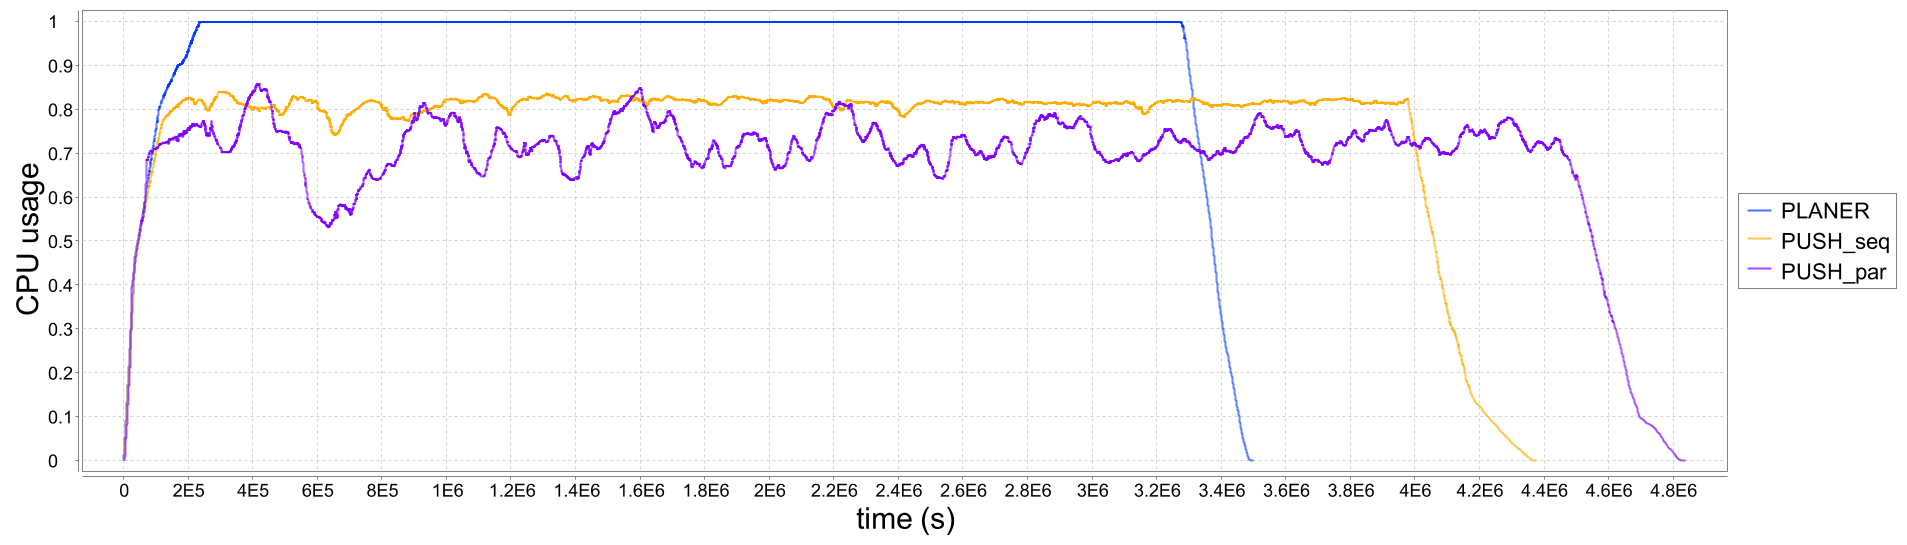
\includegraphics [trim= 0mm 00mm 0mm 00mm , clip,width=0.9\textwidth]{pic/3models_link01.png}
    \caption{Comparison of CPU usage of three models. }
      \label{multi_cpu_consumption}	
  \end{center}  
\end{figure}

The plot at Figure \ref{multi_cpu_consumption} shows the CPU utilization (percentage of busy CPUs over total CPUs in the system) as a function of time for the simulation with 100 Mbps interconnecting links. As it can be observed, both "PUSH\_par" and "PUSH\_seq" models did not manage to utilize 100\% of CPUs, and the number of busy CPUs is fluctuating over time. This simulation, also, illustrates that the currently used scheduling approach ("PUSH\_par") can lead to significant performance drop when multiple CPUs access the remote data over a shared bandwidth simultaneously and uncoordinately and, by that, delay each other. At the same time the PLANER achieves 100\% CPU utilization shortly after the start and keeps it until the end of simulation due to distributing the network load over the links which would be idle otherwise. The makespan improvement in this simulation is $\approx$ 28\% and 20\% compared to "PUSH\_par" and "PUSH\_seq" respectively .

After these simulations we can conclude that the proposed model can successfully utilize all available network capacity including indirect links in order to "preplace" data for computations. This can lead to a significant performance improvement comparing to the traditional job distribution scenarios, when data is transferred during the computation. 

\section{Conclusion}
\label{Conclusion}

In this paper we proposed a model of distributed data production, where all
the files from a single source has to be processed once and transferred back.
This model allows planning of WAN, storage and CPU loads using the network
flow maximization approach. The proposed model will enable automated and scalable planning and optimization of distributed computations which are highly required in data intensive computational fields such as High Energy and Nuclear Physics. Compared to the currently used data production scheduling the model provides three degrees of optimization: transferring data in advance before computation which allows to decrease IO latency; transferring  files sequentially in coordinated manner, which allows to reduce the influence of network bottlenecks; and load balancing over available network, which allows to split the load between several alternative transfer paths.

The model was tested using one of the standard tools for Grid simulation (GridSim). The data extracted form the log database of real data production framework of the STAR experiment at KISTI computing facility was used as input for simulations. The simulations has shown that the proposed model systematically provides better performance for distributed computations, which can reach up to 26\% compared to the current scheduling approach. According to our results, the model can help to efficiently utilize more remote computational power using a limited network bandwidth. In addition to that, the jobs are submitted to CPUs only after the data can be accessed efficiently by ones, otherwise the CPUs remain idle and can be assigned to other computational tasks. These two factors provide more flexibility when setting up a remote data production.

We continue development of the data production planer, and plan to perform simulations using data from more HENP experiments (such as ALICE at CERN) and study the effects of a background network traffic.


\begin{acknowledgements}
This work has been supported by the Czech Science Foundation
(13-20841S, P202$/$12$/$0306),  the MEYS grant CZ.1.07/2.3.00/20.0207 of the European Social Fund (ESF) in the Czech Republic: “Education for Competitiveness Operational Programme” (ECOP) and the Office of Nuclear Physics within the U.S. Department of Energy.  
\end{acknowledgements}

\bibliography{bibliography}{}
\bibliographystyle{spmpsci}

\end{document}

\end{document}
